\section{Angular Control Smoothness}
The angular control smoothness is indicated by the time differentiated control 
signal norm. Larger means less smoothness.

\begin{equation} 
     \text{Angular Control Smoothness}
     = \frac{\sum_{i=0}^{N_{end}} | \frac{\omega(t_{i+1}) - \omega(t)}{t_{i+1} - t_i} |}{N_{end}}
\end{equation}

\subsection{Short Distance Simulation Outcomes}
\vspace*{-0.5em}
\begin{figure}[H]
\begin{minipage}[t]{\textwidth}
\centering
%\vspace*{-1.45in}
\captionof{table}{ Short distance simulation angular control smoothness.\label{tab:shortCS}}
\vspace*{-0.5em}
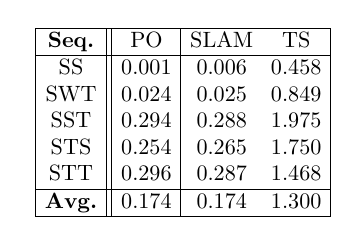
\begin{tikzpicture}[inner sep=0pt,outer sep=0pt,scale=1, every node/.style={scale=0.8}]
    % sim CS
	\node[anchor=north west] (sim_cs) at (0, 0pt)
    {
    \setlength{\tabcolsep}{4pt}
    \begin{tabular}{|c||c|cc|}
    \hline 
    \textbf{Seq.} & PO & SLAM & TS \\ 
    \hline 
%       &       &       & SLAM  & $\neg$SLAM \\
    SS  & 0.001  & 0.006  & 0.458  \\ 
    SWT & 0.024  & 0.025  & 0.849  \\ 
    SST & 0.294  & 0.288  & 1.975  \\ 
    STS & 0.254  & 0.265  & 1.750  \\ 
    STT & 0.296  & 0.287  & 1.468  \\ 
    \hline 
    \textbf{Avg.} & 0.174 & 0.174 & 1.300 \\ 
    \hline 
    \end{tabular}
    };
    
%    \node[anchor=south, text width=5cm, text centered] (sim_cs_cap) 
%    at ($(sim_cs.north) + (0pt, 2pt)$)
%    {\normalsize \textbf{(a)} Sim Angular \\ Control Smoothness};
      
%    % p-values
%    \node[anchor=west] (sim_cs_p) at ($(sim_cs.east) + (5pt, 0)$)
%    {
%    \setlength{\tabcolsep}{5pt}
%    \begin{tabular}{|l||c|}
%    \hline 
%    \textbf{PO} vs \textbf{SLAM} & 4.5e-1 \\ 
%    \hline 
%    \textbf{PO} vs \textbf{TS} & 2.6e-1 \\ 
%    \hline
%    \textbf{SLAM} vs \textbf{TS} & 2.2e-1 \\ 
%    \hline 
%    \end{tabular}
%    };
%    
%	\node[anchor=south, text width=5cm, text centered] (sim_cd_p_cap) 
%    at ($(sim_ce_p.north) + (0pt, 2pt)$)
%    {\normalsize \textbf{(b)} p-values of \\ pairwise comparisons};        

\end{tikzpicture}
\end{minipage}
\vspace*{-0.5em}
\end{figure}

\subsection{Long Distance Simulation Outcomes}
\vspace*{-0.5em}
\begin{figure}[H]
\begin{minipage}[t]{\textwidth}
\centering
%\vspace*{-1.45in}
\captionof{table}{ Long distance simulation angular control smoothness.\label{tab:longCS}}
\vspace*{-0.5em}
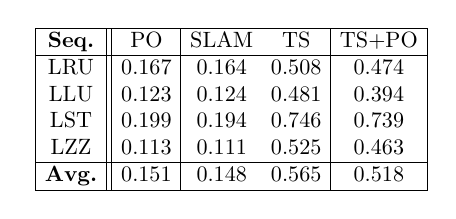
\begin{tikzpicture}[inner sep=0pt,outer sep=0pt,scale=1, every node/.style={scale=0.8}]
    % sim CS
	\node[anchor=north west] (sim_cs) at (0, 0pt)
    {
    \setlength{\tabcolsep}{4pt}
    \begin{tabular}{|c||c|cc|c|}
    \hline 
    \textbf{Seq.} & PO & SLAM & TS & TS+PO \\ 
    \hline 
%      & \textcolor{white}{$v,\omega$} & & \\
    LRU & 0.167  & 0.164  & 0.508  & 0.474 \\ 
    LLU & 0.123  & 0.124  & 0.481  & 0.394 \\ 
    LST & 0.199  & 0.194  & 0.746  & 0.739 \\ 
    LZZ & 0.113  & 0.111  & 0.525  & 0.463 \\ 
    \hline 
    \textbf{Avg.} & 0.151 & 0.148 & 0.565 & 0.518 \\
    \hline 
    \end{tabular}
    };
    
%    \node[anchor=south, text width=5cm, text centered] (sim_cs_cap) 
%    at ($(sim_cs.north) + (0pt, 2pt)$)
%    {\normalsize \textbf{(a)} Sim Angular \\ Control Smoothness};
      
%    % p-values
%    \node[anchor=west] (sim_ce_p) at ($(sim_ce.east) + (5pt, 0)$)
%    {
%    \setlength{\tabcolsep}{5pt}
%    \begin{tabular}{|l||c|}
%    \hline 
%    \textbf{PO} vs \textbf{SLAM} & 4.9e-1 \\ 
%    \hline 
%    \textbf{PO} vs \textbf{TS} & 4.4e-1 \\ 
%    \hline
%    \textbf{PO} vs \textbf{TS+PO} & 4.6e-1 \\ 
%    \hline 
%    \textbf{SLAM} vs \textbf{TS} & 4.4e-1 \\ 
%    \hline 
%    \textbf{SLAM} vs \textbf{TS+PO} & 4.6e-1 \\ 
%    \hline 
%    \textbf{TS} vs \textbf{TS+PO} & 4.8e-1 \\ 
%    \hline 
%    \end{tabular}
%    };
%    
%	\node[anchor=south, text width=5cm, text centered] (sim_ce_p_cap) 
%    at ($(sim_ce_p.north) + (0pt, 2pt)$)
%    {\normalsize \textbf{(b)} p-values of \\ pairwise comparisons};       

\end{tikzpicture}
\end{minipage}
  \vspace*{-0.5em}
\end{figure}

